\chapter{API del Servicio Web FPGA\label{extra:api_servicio_web_fpga}}

En este apéndice se detallan los métodos de la \gls{API} del \gls{servicioweb} \gls{FPGA}. Esta documentación puede también consultarse de manera interactiva (Figura \ref{fig:docsbackend}) en la propia página de la aplicación (en inglés), accediendo desde el navegador a la ruta relativa \textit{NetWatcher/docs-back-end/}. Al ser un \gls{servicioweb}, cada método se invoca mediante una llamada \gls{HTTP} \cite{httpmethods}.

Se han agrupado todos los métodos disponibles en tres categorías, coincidiendo con los módulos implementados: gestión, trazas y estadísticas. Para cada método, se especifica su ruta (relativa a la ruta del \gls{servicioweb}), los parámetros necesarios para su invocación y las posibles salidas, con un ejemplo cada una. Los parámetros se pasan por la propia \gls{URL} o en la cabecera en el caso del \textit{timestamp}. Cada método devuelve siempre un código de estado \gls{HTTP} \cite{httpcodes} y una salida en formato \gls{JSON} \cite{json}.

\begin{figure}[htp!]
  \centering
  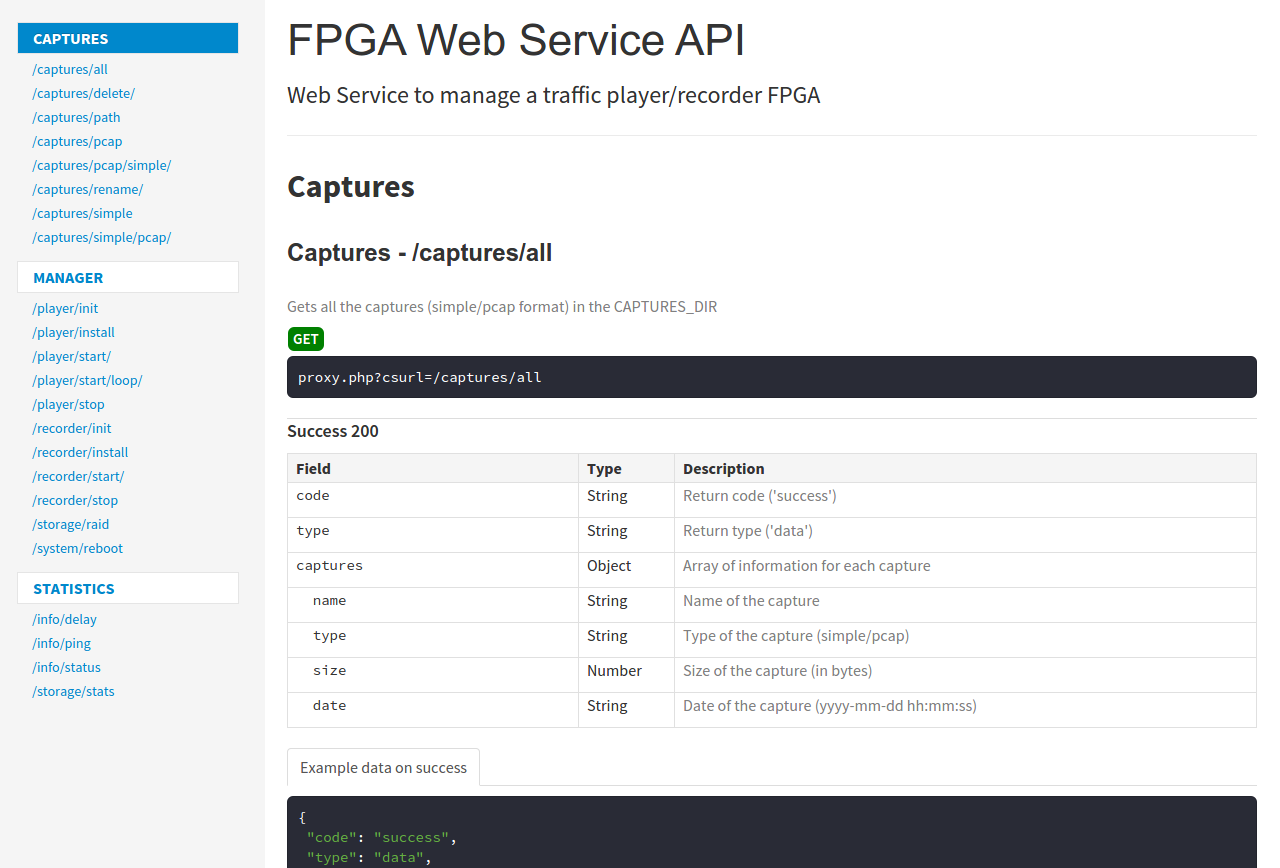
\includegraphics[width=0.95\textwidth,clip=true]{graphics/capturas/docs_back_end}
  \caption{Documentación web de la \gls{API} del \gls{servicioweb} \gls{FPGA}.}
  \label{fig:docsbackend}
\end{figure} 

\section{Métodos de Gestión \label{extra:api:gestion}}

%
% /system/reboot
%
\subsection{POST /system/reboot}

Reinicia el servidor remoto. Los parámetros necesarios para la invocación de este método se detallan en la tabla \ref{extra:api:reboot:invocacion}.

\begin{table}[H]
\centering
\begin{tabular}{|l|l|l|l|}
\hline
\rowcolor[HTML]{F5F5F5}
\textbf{Parámetro}  & \textbf{Clase} & \textbf{Tipo} & \textbf{Descripción}                  \\ \hline
                    &                &               & Tiempo transcurrido (ms) desde el 1   \\
timestamp           & Cabecera       & Número        & de Enero de 1970 00:00:00 UTC hasta   \\
                    &                &               & ahora (salida de \textit{Date.now()}) \\ \hline
\end{tabular}
\caption{Parámetros de \textit{/system/reboot}}
\label{extra:api:reboot:invocacion}
\end{table}

A continuación se enumeran los distintos códigos de retorno asociados a este método:
\begin{itemize}

\item{\textbf{200 OK:} se ha ordenado con éxito el reinicio del servidor remoto. Este código de éxito es retornado junto con los parámetros indicados en la tabla \ref{extra:api:reboot:ok}.
\begin{table}[H]
\centering
\begin{tabular}{|l|l|l|}
\hline
\rowcolor[HTML]{F5F5F5}
\textbf{Nombre}  & \textbf{Tipo}   & \textbf{Descripción}              \\ \hline
code             & Cadena de texto & Código de retorno ('success')     \\ \hline
type             & Cadena de texto & Código de tipo ('notification')   \\ \hline
description      & Cadena de texto & Descripción del código de retorno \\ \hline
\end{tabular}
\caption{Salida de \textit{/system/reboot} asociada al código 200}
\label{extra:api:reboot:ok}
\end{table}
\begin{minipage}{\textwidth}
Ejemplo de datos asociados al código 200:

\begin{code}[language=json]
{
  "code": "success",
  "type": "notification",
  "description": "The host is rebooting now."
}
\end{code}
\end{minipage}
}

\item{\textbf{412 Error:} el servidor remoto no puede ser reiniciado ya que la \gls{FPGA} está siendo usada. Este código de error es retornado junto a los parámetros indicados en la tabla \ref{extra:api:reboot:error}.
\begin{table}[H]
\centering
\begin{tabular}{|l|l|l|}
\hline
\rowcolor[HTML]{F5F5F5}
\textbf{Nombre}  & \textbf{Tipo}   & \textbf{Descripción}            \\ \hline
code             & Cadena de texto & Código de retorno ('error')     \\ \hline
type             & Cadena de texto & Código de tipo ('notification') \\ \hline
description      & Cadena de texto & Descripción del error           \\ \hline
\end{tabular}
\caption{Salida de \textit{/system/reboot} asociada al código 412}
\label{extra:api:reboot:error}
\end{table}
\begin{minipage}{\textwidth}
Ejemplo de datos asociados al código 412:

\begin{code}[language=json]
{
  "code": "error",
  "type": "notification",
  "description": "The host can not be rebooted. The FPGA is being used."
}
\end{code}
\end{minipage}
}
\end{itemize}

%
% /player/init
%
\subsection{POST /player/init}

Programa la \gls{FPGA} para reproducir \glspl{traza} y reinicia el servidor remoto. Los parámetros necesarios para la invocación de este método se detallan en la tabla \ref{extra:api:playerinit:invocacion}.

\begin{table}[H]
\centering
\begin{tabular}{|l|l|l|l|}
\hline
\rowcolor[HTML]{F5F5F5}
\textbf{Parámetro}  & \textbf{Clase} & \textbf{Tipo} & \textbf{Descripción}                  \\ \hline
                    &                &               & Tiempo transcurrido (ms) desde el 1   \\
timestamp           & Cabecera       & Número        & de Enero de 1970 00:00:00 UTC hasta   \\
                    &                &               & ahora (salida de \textit{Date.now()}) \\ \hline
\end{tabular}
\caption{Parámetros de \textit{/player/init}}
\label{extra:api:playerinit:invocacion}
\end{table}

A continuación se enumeran los distintos códigos de retorno asociados a este método:
\begin{itemize}

\item{\textbf{200 OK:} se ha programado con éxito la \gls{FPGA} para reproducir \glspl{traza} y se va a reiniciar el servidor remoto. Este código de éxito es retornado junto con los parámetros indicados en la tabla \ref{extra:api:playerinit:ok}.
\begin{table}[H]
\centering
\begin{tabular}{|l|l|l|}
\hline
\rowcolor[HTML]{F5F5F5}
\textbf{Nombre}  & \textbf{Tipo}   & \textbf{Descripción}              \\ \hline
code             & Cadena de texto & Código de retorno ('success')     \\ \hline
type             & Cadena de texto & Código de tipo ('notification')   \\ \hline
description      & Cadena de texto & Descripción del código de retorno \\ \hline
\end{tabular}
\caption{Salida de \textit{/player/init} asociada al código 200}
\label{extra:api:playerinit:ok}
\end{table}
\begin{minipage}{\textwidth}
Ejemplo de datos asociados al código 200:

\begin{code}[language=json]
{
  "code": "success",
  "type": "notification",
  "description": "The FPGA has been initialized. The host will reboot now."
}
\end{code}
\end{minipage}
}

\item{\textbf{412 Error:} la \gls{FPGA} no puede ser programada ya que está siendo usada. Este código de error es retornado junto a los parámetros indicados en la tabla \ref{extra:api:playerinit:error}.
\begin{table}[H]
\centering
\begin{tabular}{|l|l|l|}
\hline
\rowcolor[HTML]{F5F5F5}
\textbf{Nombre}  & \textbf{Tipo}   & \textbf{Descripción}                    \\ \hline
code             & Cadena de texto & Código de retorno ('error')             \\ \hline
type             & Cadena de texto & Código de tipo ('fpga\_invalid\_state') \\ \hline
description      & Cadena de texto & Descripción del error                   \\ \hline
\end{tabular}
\caption{Salida de \textit{/player/init} asociada al código 412}
\label{extra:api:playerinit:error}
\end{table}

\begin{minipage}{\textwidth}
Ejemplo de datos asociados al código 412:

\begin{code}[language=json]
{
  "code": "error",
  "type": "fpga_invalid_state",
  "description": "Invalid State. The FPGA is already running, stop it to init the FPGA."
}
\end{code}
\end{minipage}
}

\end{itemize}

%
% /recorder/init
%
\subsection{POST /recorder/init}

Programa la \gls{FPGA} para capturar \glspl{traza} y reinicia el servidor remoto. Los parámetros necesarios para la invocación de este método se detallan en la tabla \ref{extra:api:recorderinit:invocacion}.

\begin{table}[H]
\centering
\begin{tabular}{|l|l|l|l|}
\hline
\rowcolor[HTML]{F5F5F5}
\textbf{Parámetro}  & \textbf{Clase} & \textbf{Tipo} & \textbf{Descripción}                  \\ \hline
                    &                &               & Tiempo transcurrido (ms) desde el 1   \\
timestamp           & Cabecera       & Número        & de Enero de 1970 00:00:00 UTC hasta   \\
                    &                &               & ahora (salida de \textit{Date.now()}) \\ \hline
\end{tabular}
\caption{Parámetros de \textit{/recorder/init}}
\label{extra:api:recorderinit:invocacion}
\end{table}

A continuación se enumeran los distintos códigos de retorno asociados a este método:
\begin{itemize}

\item{\textbf{200 OK:} se ha programado con éxito la \gls{FPGA} para reproducir \glspl{traza} y se va a reiniciar el servidor remoto. Este código de éxito es retornado junto con los parámetros indicados en la tabla \ref{extra:api:recorderinit:ok}.
\begin{table}[H]
\centering
\begin{tabular}{|l|l|l|}
\hline
\rowcolor[HTML]{F5F5F5}
\textbf{Nombre}  & \textbf{Tipo}   & \textbf{Descripción}              \\ \hline
code             & Cadena de texto & Código de retorno ('success')     \\ \hline
type             & Cadena de texto & Código de tipo ('notification')   \\ \hline
description      & Cadena de texto & Descripción del código de retorno \\ \hline
\end{tabular}
\caption{Salida de \textit{/recorder/init} asociada al código 200}
\label{extra:api:recorderinit:ok}
\end{table}
\begin{minipage}{\textwidth}
Ejemplo de datos asociados al código 200:

\begin{code}[language=json]
{
  "code": "success",
  "type": "notification",
  "description": "The FPGA has been initialized. The host will reboot now."
}
\end{code}
\end{minipage}
}

\item{\textbf{412 Error:} la \gls{FPGA} no puede ser programada ya que está siendo usada. Este código de error es retornado junto a los parámetros indicados en la tabla \ref{extra:api:recorderinit:error}.
\begin{table}[H]
\centering
\begin{tabular}{|l|l|l|}
\hline
\rowcolor[HTML]{F5F5F5}
\textbf{Nombre}  & \textbf{Tipo}   & \textbf{Descripción}                    \\ \hline
code             & Cadena de texto & Código de retorno ('error')             \\ \hline
type             & Cadena de texto & Código de tipo ('fpga\_invalid\_state') \\ \hline
description      & Cadena de texto & Descripción del error                   \\ \hline
\end{tabular}
\caption{Salida de \textit{/recorder/init} asociada al código 412}
\label{extra:api:recorderinit:error}
\end{table}

\begin{minipage}{\textwidth}
Ejemplo de datos asociados al código 412:

\begin{code}[language=json]
{
  "code": "error",
  "type": "fpga_invalid_state",
  "description": "Invalid State. The FPGA is already running, stop it to init the FPGA."
}
\end{code}
\end{minipage}
}

\end{itemize}

%
% /player/install
%
\subsection{POST /player/install}
Instala y monta la \gls{FPGA} para reproducir \glspl{traza}. Los parámetros necesarios para la invocación de este método se detallan en la tabla \ref{extra:api:playerinstall:invocacion}.

\begin{table}[H]
\centering
\begin{tabular}{|l|l|l|l|}
\hline
\rowcolor[HTML]{F5F5F5}
\textbf{Parámetro}  & \textbf{Clase} & \textbf{Tipo} & \textbf{Descripción}                  \\ \hline
                    &                &               & Tiempo transcurrido (ms) desde el 1   \\
timestamp           & Cabecera       & Número        & de Enero de 1970 00:00:00 UTC hasta   \\
                    &                &               & ahora (salida de \textit{Date.now()}) \\ \hline
\end{tabular}
\caption{Parámetros de \textit{/player/install}}
\label{extra:api:playerinstall:invocacion}
\end{table}

A continuación se enumeran los distintos códigos de retorno asociados a este método:
\begin{itemize}

\item{\textbf{200 OK:} la \gls{FPGA} se ha instalado y montado con éxito, y está lista para reproducir \glspl{traza}. Este código de éxito es retornado junto con los parámetros indicados en la tabla \ref{extra:api:playerinstall:ok}.
\begin{table}[H]
\centering
\begin{tabular}{|l|l|l|}
\hline
\rowcolor[HTML]{F5F5F5}
\textbf{Nombre}  & \textbf{Tipo}   & \textbf{Descripción}              \\ \hline
code             & Cadena de texto & Código de retorno ('success')     \\ \hline
type             & Cadena de texto & Código de tipo ('notification')   \\ \hline
description      & Cadena de texto & Descripción del código de retorno \\ \hline
\end{tabular}
\caption{Salida de \textit{/player/install} asociada al código 200}
\label{extra:api:playerinstall:ok}
\end{table}
\begin{minipage}{\textwidth}
Ejemplo de datos asociados al código 200:

\begin{code}[language=json]
{
  "code": "success",
  "type": "notification",
  "description": "The FPGA has been mounted and is ready to be used."
}
\end{code}
\end{minipage}
}

\item{\textbf{412 Error:} la \gls{FPGA} no puede ser instalada y montada ya que no ha sido programada. Este código de error es retornado junto a los parámetros indicados en la tabla \ref{extra:api:playerinstall:error}.
\begin{table}[H]
\centering
\begin{tabular}{|l|l|l|}
\hline
\rowcolor[HTML]{F5F5F5}
\textbf{Nombre}  & \textbf{Tipo}   & \textbf{Descripción}                    \\ \hline
code             & Cadena de texto & Código de retorno ('error')             \\ \hline
type             & Cadena de texto & Código de tipo ('fpga\_invalid\_state') \\ \hline
description      & Cadena de texto & Descripción del error                   \\ \hline
\end{tabular}
\caption{Salida de \textit{/player/install} asociada al código 412}
\label{extra:api:playerinstall:error}
\end{table}

\begin{minipage}{\textwidth}
Ejemplo de datos asociados al código 412:

\begin{code}[language=json]
{
  "code": "error",
  "type": "fpga_invalid_state",
  "description": "Invalid State. The FPGA must be programmed before mounted."
}
\end{code}
\end{minipage}
}

\end{itemize}

%
% /recorder/install
%
\subsection{POST /recorder/install}
Instala y monta la \gls{FPGA} para capturar \glspl{traza}. Los parámetros necesarios para la invocación de este método se detallan en la tabla \ref{extra:api:recorderinstall:invocacion}.

\begin{table}[H]
\centering
\begin{tabular}{|l|l|l|l|}
\hline
\rowcolor[HTML]{F5F5F5}
\textbf{Parámetro}  & \textbf{Clase} & \textbf{Tipo} & \textbf{Descripción}                  \\ \hline
                    &                &               & Tiempo transcurrido (ms) desde el 1   \\
timestamp           & Cabecera       & Número        & de Enero de 1970 00:00:00 UTC hasta   \\
                    &                &               & ahora (salida de \textit{Date.now()}) \\ \hline
\end{tabular}
\caption{Parámetros de \textit{/recorder/install}}
\label{extra:api:recorderinstall:invocacion}
\end{table}

A continuación se enumeran los distintos códigos de retorno asociados a este método:
\begin{itemize}

\item{\textbf{200 OK:} la \gls{FPGA} se ha instalado y montado con éxito, y está lista para capturar \glspl{traza}. Este código de éxito es retornado junto con los parámetros indicados en la tabla \ref{extra:api:recorderinstall:ok}.
\begin{table}[H]
\centering
\begin{tabular}{|l|l|l|}
\hline
\rowcolor[HTML]{F5F5F5}
\textbf{Nombre}  & \textbf{Tipo}   & \textbf{Descripción}              \\ \hline
code             & Cadena de texto & Código de retorno ('success')     \\ \hline
type             & Cadena de texto & Código de tipo ('notification')   \\ \hline
description      & Cadena de texto & Descripción del código de retorno \\ \hline
\end{tabular}
\caption{Salida de \textit{/recorder/install} asociada al código 200}
\label{extra:api:recorderinstall:ok}
\end{table}
\begin{minipage}{\textwidth}
Ejemplo de datos asociados al código 200:

\begin{code}[language=json]
{
  "code": "success",
  "type": "notification",
  "description": "The FPGA has been mounted and is ready to be used."
}
\end{code}
\end{minipage}
}

\item{\textbf{412 Error:} la \gls{FPGA} no puede ser instalada y montada ya que no ha sido programada. Este código de error es retornado junto a los parámetros indicados en la tabla \ref{extra:api:recorderinstall:error}.
\begin{table}[H]
\centering
\begin{tabular}{|l|l|l|}
\hline
\rowcolor[HTML]{F5F5F5}
\textbf{Nombre}  & \textbf{Tipo}   & \textbf{Descripción}                    \\ \hline
code             & Cadena de texto & Código de retorno ('error')             \\ \hline
type             & Cadena de texto & Código de tipo ('fpga\_invalid\_state') \\ \hline
description      & Cadena de texto & Descripción del error                   \\ \hline
\end{tabular}
\caption{Salida de \textit{/recorder/install} asociada al código 412}
\label{extra:api:recorderinstall:error}
\end{table}

\begin{minipage}{\textwidth}
Ejemplo de datos asociados al código 412:

\begin{code}[language=json]
{
  "code": "error",
  "type": "fpga_invalid_state",
  "description": "Invalid State. The FPGA must be programmed before mounted."
}
\end{code}
\end{minipage}
}

\end{itemize}

%
% /player/start/:capturename/:mask/:ifg
%
\subsection{POST /player/start/:capturename/:mask/:ifg}
Reproduce una \gls{traza} con los parámetros indicados. Los parámetros necesarios para la invocación de este método se detallan en la tabla \ref{extra:api:playerstart:invocacion}.

\begin{table}[H]
\centering
\begin{tabular}{|l|l|l|l|}
\hline
\rowcolor[HTML]{F5F5F5}
\textbf{Parámetro}  & \textbf{Clase} & \textbf{Tipo}   & \textbf{Descripción}                        \\ \hline
                    &                &                 & Tiempo transcurrido (ms) desde el           \\
timestamp           & Cabecera       & Número          & 1 de Enero de 1970 00:00:00 UTC             \\
                    &                &                 & hasta ahora (salida de \textit{Date.now()}) \\ \hline
capturename         & Parámetro URL  & Cadena de texto & Nombre de la \gls{traza} a reproducir       \\ \hline
mask                & Parámetro URL  & Número          & Máscara de reproducción (0-1-2-3)           \\ \hline
ifg                 & Parámetro URL  & Número          & \gls{IFG} (0 para tasa original)            \\ \hline
\end{tabular}
\caption{Parámetros de \textit{/player/start}}
\label{extra:api:playerstart:invocacion}
\end{table}

A continuación se enumeran los distintos códigos de retorno asociados a este método:
\begin{itemize}

\item{\textbf{200 OK:} la \gls{FPGA} ha empezado a reproducir la \gls{traza} seleccionada con los parámetros indicados. Este código de éxito es retornado junto con los parámetros indicados en la tabla \ref{extra:api:playerstart:ok}.
\begin{table}[H]
\centering
\begin{tabular}{|l|l|l|}
\hline
\rowcolor[HTML]{F5F5F5}
\textbf{Nombre}  & \textbf{Tipo}   & \textbf{Descripción}              \\ \hline
code             & Cadena de texto & Código de retorno ('success')     \\ \hline
type             & Cadena de texto & Código de tipo ('notification')   \\ \hline
description      & Cadena de texto & Descripción del código de retorno \\ \hline
\end{tabular}
\caption{Salida de \textit{/player/start} asociada al código 200}
\label{extra:api:playerstart:ok}
\end{table}
\begin{minipage}{\textwidth}
Ejemplo de datos asociados al código 200:

\begin{code}[language=json]
{
  "code": "success",
  "type": "notification",
  "description": "The FPGA has started playing a capture."
}
\end{code}
\end{minipage}
}

\item{\textbf{400 Error:} la \gls{FPGA} no puede reproducir la \gls{traza} ya que los parámetros pasados son inválidos. Este código de error es retornado junto a los parámetros indicados en la tabla \ref{extra:api:playerstart:error400}.
\begin{table}[H]
\centering
\begin{tabular}{|l|l|l|}
\hline
\rowcolor[HTML]{F5F5F5}
\textbf{Nombre}  & \textbf{Tipo}   & \textbf{Descripción}                    \\ \hline
code             & Cadena de texto & Código de retorno ('error')             \\ \hline
type             & Cadena de texto & Código de tipo ('fpga\_invalid\_state') \\ \hline
description      & Cadena de texto & Descripción del error                   \\ \hline
\end{tabular}
\caption{Salida de \textit{/player/start} asociada al código 400}
\label{extra:api:playerstart:error400}
\end{table}

\begin{minipage}{\textwidth}
Ejemplo de datos asociados al código 400:

\begin{code}[language=json]
{
  "code": "error",
  "type": "notification",
  "description": "Invalid parameters. The FPGA could not start playing a capture."
}
\end{code}
\end{minipage}
}

\item{\textbf{412 Error:} la \gls{FPGA} no puede reproducir la \gls{traza} ya que no ha sido instalada y montada para reproducir \glspl{traza}. Este código de error es retornado junto a los parámetros indicados en la tabla \ref{extra:api:playerstart:error412}.
\begin{table}[H]
\centering
\begin{tabular}{|l|l|l|}
\hline
\rowcolor[HTML]{F5F5F5}
\textbf{Nombre}  & \textbf{Tipo}   & \textbf{Descripción}                    \\ \hline
code             & Cadena de texto & Código de retorno ('error')             \\ \hline
type             & Cadena de texto & Código de tipo ('fpga\_invalid\_state') \\ \hline
description      & Cadena de texto & Descripción del error                   \\ \hline
\end{tabular}
\caption{Salida de \textit{/player/start} asociada al código 412}
\label{extra:api:playerstart:error412}
\end{table}

\begin{minipage}{\textwidth}
Ejemplo de datos asociados al código 412:

\begin{code}[language=json]
{
  "code": "error",
  "type": "fpga_invalid_state",
  "description": "Invalid State. The FPGA is not programmed and mounted as a player."
}
\end{code}
\end{minipage}
}

\end{itemize}

%
% /player/start/loop/:capturename/:mask/:ifg
%
\subsection{POST /player/start/loop/:capturename/:mask/:ifg}
Reproduce en bucle una \gls{traza} con los parámetros indicados. Los parámetros necesarios para la invocación de este método se detallan en la tabla \ref{extra:api:playerstartloop:invocacion}.

\begin{table}[H]
\centering
\begin{tabular}{|l|l|l|l|}
\hline
\rowcolor[HTML]{F5F5F5}
\textbf{Parámetro}  & \textbf{Clase} & \textbf{Tipo}   & \textbf{Descripción}                        \\ \hline
                    &                &                 & Tiempo transcurrido (ms) desde el           \\
timestamp           & Cabecera       & Número          & 1 de Enero de 1970 00:00:00 UTC             \\
                    &                &                 & hasta ahora (salida de \textit{Date.now()}) \\ \hline
capturename         & Parámetro URL  & Cadena de texto & Nombre de la \gls{traza} a reproducir       \\ \hline
mask                & Parámetro URL  & Número          & Máscara de reproducción (0-1-2-3)           \\ \hline
ifg                 & Parámetro URL  & Número          & \gls{IFG} (0 para tasa original)            \\ \hline
\end{tabular}
\caption{Parámetros de \textit{/player/start/loop}}
\label{extra:api:playerstartloop:invocacion}
\end{table}

A continuación se enumeran los distintos códigos de retorno asociados a este método:
\begin{itemize}

\item{\textbf{200 OK:} la \gls{FPGA} ha empezado a reproducir en bucle la \gls{traza} seleccionada con los parámetros indicados. Este código de éxito es retornado junto con los parámetros indicados en la tabla \ref{extra:api:playerstartloop:ok}.
\begin{table}[H]
\centering
\begin{tabular}{|l|l|l|}
\hline
\rowcolor[HTML]{F5F5F5}
\textbf{Nombre}  & \textbf{Tipo}   & \textbf{Descripción}              \\ \hline
code             & Cadena de texto & Código de retorno ('success')     \\ \hline
type             & Cadena de texto & Código de tipo ('notification')   \\ \hline
description      & Cadena de texto & Descripción del código de retorno \\ \hline
\end{tabular}
\caption{Salida de \textit{/player/start/loop} asociada al código 200}
\label{extra:api:playerstartloop:ok}
\end{table}
\begin{minipage}{\textwidth}
Ejemplo de datos asociados al código 200:

\begin{code}[language=json]
{
  "code": "success",
  "type": "notification",
  "description": "The FPGA has started playing a capture."
}
\end{code}
\end{minipage}
}

\item{\textbf{400 Error:} la \gls{FPGA} no puede reproducir la \gls{traza} ya que los parámetros pasados son inválidos. Este código de error es retornado junto a los parámetros indicados en la tabla \ref{extra:api:playerstartloop:error400}.
\begin{table}[H]
\centering
\begin{tabular}{|l|l|l|}
\hline
\rowcolor[HTML]{F5F5F5}
\textbf{Nombre}  & \textbf{Tipo}   & \textbf{Descripción}                    \\ \hline
code             & Cadena de texto & Código de retorno ('error')             \\ \hline
type             & Cadena de texto & Código de tipo ('fpga\_invalid\_state') \\ \hline
description      & Cadena de texto & Descripción del error                   \\ \hline
\end{tabular}
\caption{Salida de \textit{/player/start/loop} asociada al código 400}
\label{extra:api:playerstartloop:error400}
\end{table}

\begin{minipage}{\textwidth}
Ejemplo de datos asociados al código 400:

\begin{code}[language=json]
{
  "code": "error",
  "type": "notification",
  "description": "Invalid parameters. The FPGA could not start playing a capture."
}
\end{code}
\end{minipage}
}

\item{\textbf{412 Error:} la \gls{FPGA} no puede reproducir la \gls{traza} ya que no ha sido instalada y montada para reproducir \glspl{traza}. Este código de error es retornado junto a los parámetros indicados en la tabla \ref{extra:api:playerstartloop:error412}.
\begin{table}[H]
\centering
\begin{tabular}{|l|l|l|}
\hline
\rowcolor[HTML]{F5F5F5}
\textbf{Nombre}  & \textbf{Tipo}   & \textbf{Descripción}                    \\ \hline
code             & Cadena de texto & Código de retorno ('error')             \\ \hline
type             & Cadena de texto & Código de tipo ('fpga\_invalid\_state') \\ \hline
description      & Cadena de texto & Descripción del error                   \\ \hline
\end{tabular}
\caption{Salida de \textit{/player/start/loop} asociada al código 412}
\label{extra:api:playerstartloop:error412}
\end{table}

\begin{minipage}{\textwidth}
Ejemplo de datos asociados al código 412:

\begin{code}[language=json]
{
  "code": "error",
  "type": "fpga_invalid_state",
  "description": "Invalid State. The FPGA is not programmed and mounted as a player."
}
\end{code}
\end{minipage}
}

\end{itemize}

%
% /recorder/start/:capturename/:port/:bytes
%
\subsection{POST /recorder/start/:capturename/:port/:bytes}
Captura una \gls{traza} con los parámetros indicados. Los parámetros necesarios para la invocación de este método se detallan en la tabla \ref{extra:api:recorderstart:invocacion}.

\begin{table}[H]
\centering
\begin{tabular}{|l|l|l|l|}
\hline
\rowcolor[HTML]{F5F5F5}
\textbf{Parámetro}  & \textbf{Clase} & \textbf{Tipo}   & \textbf{Descripción}                         \\ \hline
                    &                &                 & Tiempo transcurrido (ms) desde el            \\
timestamp           & Cabecera       & Número          & 1 de Enero de 1970 00:00:00 UTC              \\
                    &                &                 & hasta ahora (salida de \textit{Date.now()})  \\ \hline
capturename         & Parámetro URL  & Cadena de texto & Nombre de la \gls{traza} a capturar          \\ \hline
port                & Parámetro URL  & Número          & Puerto a capturar (0-1-2-3)                  \\ \hline
bytes               & Parámetro URL  & Número          & Bytes a capturar                             \\ \hline
\end{tabular}
\caption{Parámetros de \textit{/recorder/start}}
\label{extra:api:recorderstart:invocacion}
\end{table}

A continuación se enumeran los distintos códigos de retorno asociados a este método:
\begin{itemize}

\item{\textbf{200 OK:} la \gls{FPGA} ha empezado a capturar una traza con los parámetros indicados. Este código de éxito es retornado junto con los parámetros indicados en la tabla \ref{extra:api:recorderstart:ok}.
\begin{table}[H]
\centering
\begin{tabular}{|l|l|l|}
\hline
\rowcolor[HTML]{F5F5F5}
\textbf{Nombre}  & \textbf{Tipo}   & \textbf{Descripción}              \\ \hline
code             & Cadena de texto & Código de retorno ('success')     \\ \hline
type             & Cadena de texto & Código de tipo ('notification')   \\ \hline
description      & Cadena de texto & Descripción del código de retorno \\ \hline
\end{tabular}
\caption{Salida de \textit{/recorder/start} asociada al código 200}
\label{extra:api:recorderstart:ok}
\end{table}
\begin{minipage}{\textwidth}
Ejemplo de datos asociados al código 200:

\begin{code}[language=json]
{
  "code": "success",
  "type": "notification",
  "description": "The FPGA has started recording data."
}
\end{code}
\end{minipage}
}

\item{\textbf{400 Error:} la \gls{FPGA} no puede empezar a capturar ya que los parámetros pasados son inválidos. Este código de error es retornado junto a los parámetros indicados en la tabla \ref{extra:api:recorderstart:error400}.
\begin{table}[H]
\centering
\begin{tabular}{|l|l|l|}
\hline
\rowcolor[HTML]{F5F5F5}
\textbf{Nombre}  & \textbf{Tipo}   & \textbf{Descripción}                    \\ \hline
code             & Cadena de texto & Código de retorno ('error')             \\ \hline
type             & Cadena de texto & Código de tipo ('fpga\_invalid\_state') \\ \hline
description      & Cadena de texto & Descripción del error                   \\ \hline
\end{tabular}
\caption{Salida de \textit{/recorder/start} asociada al código 400}
\label{extra:api:recorderstart:error400}
\end{table}

\begin{minipage}{\textwidth}
Ejemplo de datos asociados al código 400:

\begin{code}[language=json]
{
  "code": "error",
  "type": "notification",
  "description": "Invalid capture name (must not exist)."
}
\end{code}
\end{minipage}
}

\item{\textbf{412 Error:} la \gls{FPGA} no puede empezar a capturar ya que no ha sido instalada y montada para capturar \glspl{traza}. Este código de error es retornado junto a los parámetros indicados en la tabla \ref{extra:api:recorderstart:error412}.
\begin{table}[H]
\centering
\begin{tabular}{|l|l|l|}
\hline
\rowcolor[HTML]{F5F5F5}
\textbf{Nombre}  & \textbf{Tipo}   & \textbf{Descripción}                    \\ \hline
code             & Cadena de texto & Código de retorno ('error')             \\ \hline
type             & Cadena de texto & Código de tipo ('fpga\_invalid\_state') \\ \hline
description      & Cadena de texto & Descripción del error                   \\ \hline
\end{tabular}
\caption{Salida de \textit{/recorder/start} asociada al código 412}
\label{extra:api:recorderstart:error412}
\end{table}

\begin{minipage}{\textwidth}
Ejemplo de datos asociados al código 412:

\begin{code}[language=json]
{
  "code": "error",
  "type": "fpga_invalid_state",
  "description": "Invalid State. The FPGA is not programmed and mounted as a recorder."
}
\end{code}
\end{minipage}
}

\end{itemize}

%
% /player/stop
%
\subsection{POST /player/stop}
Para la reproducción de \gls{traza} en curso. Los parámetros necesarios para la invocación de este método se detallan en la tabla \ref{extra:api:playerstop:invocacion}.

\begin{table}[H]
\centering
\begin{tabular}{|l|l|l|l|}
\hline
\rowcolor[HTML]{F5F5F5}
\textbf{Parámetro}  & \textbf{Clase} & \textbf{Tipo}   & \textbf{Descripción}                         \\ \hline
                    &                &                 & Tiempo transcurrido (ms) desde el            \\
timestamp           & Cabecera       & Número          & 1 de Enero de 1970 00:00:00 UTC              \\
                    &                &                 & hasta ahora (salida de \textit{Date.now()})  \\ \hline
\end{tabular}
\caption{Parámetros de \textit{/player/stop}}
\label{extra:api:playerstop:invocacion}
\end{table}

A continuación se enumeran los distintos códigos de retorno asociados a este método:
\begin{itemize}

\item{\textbf{200 OK:} la \gls{FPGA} ha detenido la reproducción en curso. Este código de éxito es retornado junto con los parámetros indicados en la tabla \ref{extra:api:playerstop:ok}.
\begin{table}[H]
\centering
\begin{tabular}{|l|l|l|}
\hline
\rowcolor[HTML]{F5F5F5}
\textbf{Nombre}  & \textbf{Tipo}   & \textbf{Descripción}              \\ \hline
code             & Cadena de texto & Código de retorno ('success')     \\ \hline
type             & Cadena de texto & Código de tipo ('notification')   \\ \hline
description      & Cadena de texto & Descripción del código de retorno \\ \hline
\end{tabular}
\caption{Salida de \textit{/player/stop} asociada al código 200}
\label{extra:api:playerstop:ok}
\end{table}
\begin{minipage}{\textwidth}
Ejemplo de datos asociados al código 200:

\begin{code}[language=json]
{
  "code": "success",
  "type": "notification",
  "description": "The FPGA has stopped playing a capture."
}
\end{code}
\end{minipage}
}

\item{\textbf{412 Error:} no se ha podido detener la reproducción ya que no existe ninguna en curso. Este código de error es retornado junto a los parámetros indicados en la tabla \ref{extra:api:playerstop:error}.
\begin{table}[H]
\centering
\begin{tabular}{|l|l|l|}
\hline
\rowcolor[HTML]{F5F5F5}
\textbf{Nombre}  & \textbf{Tipo}   & \textbf{Descripción}                    \\ \hline
code             & Cadena de texto & Código de retorno ('error')             \\ \hline
type             & Cadena de texto & Código de tipo ('fpga\_invalid\_state') \\ \hline
description      & Cadena de texto & Descripción del error                   \\ \hline
\end{tabular}
\caption{Salida de \textit{/player/stop} asociada al código 412}
\label{extra:api:playerstop:error}
\end{table}

\begin{minipage}{\textwidth}
Ejemplo de datos asociados al código 412:

\begin{code}[language=json]
{
  "code": "error",
  "type": "fpga_invalid_state",
  "description": "Invalid State. The FPGA is not playing a capture."
}
\end{code}
\end{minipage}
}

\end{itemize}

%
% /recorder/stop
%
\subsection{POST /recorder/stop}
Para la captura de \gls{traza} en curso. Los parámetros necesarios para la invocación de este método se detallan en la tabla \ref{extra:api:recorderstop:invocacion}.

\begin{table}[H]
\centering
\begin{tabular}{|l|l|l|l|}
\hline
\rowcolor[HTML]{F5F5F5}
\textbf{Parámetro}  & \textbf{Clase} & \textbf{Tipo}   & \textbf{Descripción}                         \\ \hline
                    &                &                 & Tiempo transcurrido (ms) desde el            \\
timestamp           & Cabecera       & Número          & 1 de Enero de 1970 00:00:00 UTC              \\
                    &                &                 & hasta ahora (salida de \textit{Date.now()})  \\ \hline
\end{tabular}
\caption{Parámetros de \textit{/recorder/stop}}
\label{extra:api:recorderstop:invocacion}
\end{table}

A continuación se enumeran los distintos códigos de retorno asociados a este método:
\begin{itemize}

\item{\textbf{200 OK:} la \gls{FPGA} ha detenido la captura en curso. Este código de éxito es retornado junto con los parámetros indicados en la tabla \ref{extra:api:recorderstop:ok}.
\begin{table}[H]
\centering
\begin{tabular}{|l|l|l|}
\hline
\rowcolor[HTML]{F5F5F5}
\textbf{Nombre}  & \textbf{Tipo}   & \textbf{Descripción}              \\ \hline
code             & Cadena de texto & Código de retorno ('success')     \\ \hline
type             & Cadena de texto & Código de tipo ('notification')   \\ \hline
description      & Cadena de texto & Descripción del código de retorno \\ \hline
\end{tabular}
\caption{Salida de \textit{/recorder/stop} asociada al código 200}
\label{extra:api:recorderstop:ok}
\end{table}
\begin{minipage}{\textwidth}
Ejemplo de datos asociados al código 200:

\begin{code}[language=json]
{
  "code": "success",
  "type": "notification",
  "description": "The FPGA has stopped recording data."
}
\end{code}
\end{minipage}
}

\item{\textbf{412 Error:} no se ha podido detener la captura ya que no existe ninguna en curso. Este código de error es retornado junto a los parámetros indicados en la tabla \ref{extra:api:recorderstop:error}.
\begin{table}[H]
\centering
\begin{tabular}{|l|l|l|}
\hline
\rowcolor[HTML]{F5F5F5}
\textbf{Nombre}  & \textbf{Tipo}   & \textbf{Descripción}                    \\ \hline
code             & Cadena de texto & Código de retorno ('error')             \\ \hline
type             & Cadena de texto & Código de tipo ('fpga\_invalid\_state') \\ \hline
description      & Cadena de texto & Descripción del error                   \\ \hline
\end{tabular}
\caption{Salida de \textit{/recorder/stop} asociada al código 412}
\label{extra:api:recorderstop:error}
\end{table}

\begin{minipage}{\textwidth}
Ejemplo de datos asociados al código 412:

\begin{code}[language=json]
{
  "code": "error",
  "type": "fpga_invalid_state",
  "description": "Invalid State. The FPGA is not recording data."
}
\end{code}
\end{minipage}
}

\end{itemize}

%
% /storage/raid
%
\subsection{DELETE /storage/raid}
Borra (formatea y vuelve a crear) el \gls{RAID} de almacenamiento. Los parámetros necesarios para la invocación de este método se detallan en la tabla \ref{extra:api:storageraid:invocacion}.

\begin{table}[H]
\centering
\begin{tabular}{|l|l|l|l|}
\hline
\rowcolor[HTML]{F5F5F5}
\textbf{Parámetro}  & \textbf{Clase} & \textbf{Tipo}   & \textbf{Descripción}                         \\ \hline
                    &                &                 & Tiempo transcurrido (ms) desde el            \\
timestamp           & Cabecera       & Número          & 1 de Enero de 1970 00:00:00 UTC              \\
                    &                &                 & hasta ahora (salida de \textit{Date.now()})  \\ \hline
\end{tabular}
\caption{Parámetros de \textit{/storage/raid}}
\label{extra:api:storageraid:invocacion}
\end{table}

A continuación se enumeran los distintos códigos de retorno asociados a este método:
\begin{itemize}

\item{\textbf{200 OK:} se ha formateado y vuelto a montar el \gls{RAID} de almacenamiento. Este código de éxito es retornado junto con los parámetros indicados en la tabla \ref{extra:api:storageraid:ok}.
\begin{table}[H]
\centering
\begin{tabular}{|l|l|l|}
\hline
\rowcolor[HTML]{F5F5F5}
\textbf{Nombre}  & \textbf{Tipo}   & \textbf{Descripción}              \\ \hline
code             & Cadena de texto & Código de retorno ('success')     \\ \hline
type             & Cadena de texto & Código de tipo ('notification')   \\ \hline
description      & Cadena de texto & Descripción del código de retorno \\ \hline
\end{tabular}
\caption{Salida de \textit{/storage/raid} asociada al código 200}
\label{extra:api:storageraid:ok}
\end{table}
\begin{minipage}{\textwidth}
Ejemplo de datos asociados al código 200:

\begin{code}[language=json]
{
  "code": "success",
  "type": "notification",
  "description": "The RAID has been formatted and mounted properly."
}
\end{code}
\end{minipage}
}

\item{\textbf{412 Error:} no se ha formateado el \gls{RAID} ya que o está activado o la \gls{FPGA} está en uso. Este código de error es retornado junto a los parámetros indicados en la tabla \ref{extra:api:storageraid:error}.
\begin{table}[H]
\centering
\begin{tabular}{|l|l|l|}
\hline
\rowcolor[HTML]{F5F5F5}
\textbf{Nombre}  & \textbf{Tipo}   & \textbf{Descripción}                    \\ \hline
code             & Cadena de texto & Código de retorno ('error')             \\ \hline
type             & Cadena de texto & Código de tipo ('fpga\_invalid\_state') \\ \hline
description      & Cadena de texto & Descripción del error                   \\ \hline
\end{tabular}
\caption{Salida de \textit{/storage/raid} asociada al código 412}
\label{extra:api:storageraid:error}
\end{table}

\begin{minipage}{\textwidth}
Ejemplo de datos asociados al código 412:

\begin{code}[language=json]
{
  "code": "error",
  "type": "notification",
  "description": "The RAID could not be formatted, RAID configuration option is not set or the FPGA is running."
}
\end{code}
\end{minipage}
}

\end{itemize}



\section{Métodos de Estadísticas \label{extra:api:estadisticas}}

%
% /info/ping
%
\subsection{GET /info/ping}
Método para comprobar si el servidor está operativo. Este método no requiere parámetros.

A continuación se enumeran los distintos códigos de retorno asociados a este método:
\begin{itemize}

\item{\textbf{200 OK:} servidor operativo. Este código de éxito es retornado junto con los parámetros indicados en la tabla \ref{extra:api:infoping:ok}.
\begin{table}[H]
\centering
\begin{tabular}{|l|l|l|}
\hline
\rowcolor[HTML]{F5F5F5}
\textbf{Nombre}  & \textbf{Tipo}   & \textbf{Descripción}              \\ \hline
code             & Cadena de texto & Código de retorno ('success')     \\ \hline
\end{tabular}
\caption{Salida de \textit{/info/ping} asociada al código 200}
\label{extra:api:infoping:ok}
\end{table}
\begin{minipage}{\textwidth}
Ejemplo de datos asociados al código 200:

\begin{code}[language=json]
{
  "code": "success"
}
\end{code}
\end{minipage}
}

\end{itemize}

%
% /info/delay
%
\subsection{GET /info/delay}
Solicita la diferencia de tiempos existente entre los relojes del cliente y del servidor (en segundos). Los parámetros necesarios para la invocación de este método se detallan en la tabla \ref{extra:api:infodelay:invocacion}.

\begin{table}[H]
\centering
\begin{tabular}{|l|l|l|l|}
\hline
\rowcolor[HTML]{F5F5F5}
\textbf{Parámetro}  & \textbf{Clase} & \textbf{Tipo}   & \textbf{Descripción}                         \\ \hline
                    &                &                 & Tiempo transcurrido (ms) desde el            \\
timestamp           & Cabecera       & Número          & 1 de Enero de 1970 00:00:00 UTC              \\
                    &                &                 & hasta ahora (salida de \textit{Date.now()})  \\ \hline
\end{tabular}
\caption{Parámetros de \textit{/info/delay}}
\label{extra:api:infodelay:invocacion}
\end{table}

A continuación se enumeran los distintos códigos de retorno asociados a este método:
\begin{itemize}

\item{\textbf{200 OK:} solicitud con éxito. Este código de éxito es retornado junto con los parámetros indicados en la tabla \ref{extra:api:infodelay:ok}.
\begin{table}[H]
\centering
\begin{tabular}{|l|l|l|}
\hline
\rowcolor[HTML]{F5F5F5}
\textbf{Nombre}  & \textbf{Tipo}   & \textbf{Descripción}                      \\ \hline
code             & Cadena de texto & Código de retorno ('success')             \\ \hline
type             & Cadena de texto & Código de tipo ('data')                   \\ \hline
delay            & Número          & Diferencia entre relojes (en segundos)    \\ \hline
maxDelay         & Número          & Máxima diferencia permitida (en segundos) \\ \hline
\end{tabular}
\caption{Salida de \textit{/info/delay} asociada al código 200}
\label{extra:api:infodelay:ok}
\end{table}
\begin{minipage}{\textwidth}
Ejemplo de datos asociados al código 200:

\begin{code}[language=json]
 {
   "code": "success",
   "type": "data",
   "delay": 1,
   "maxDelay": 30
 }
\end{code}
\end{minipage}
}

\end{itemize}

%
% /info/status
%
\subsection{GET /info/status}
Solicita el estado actual de la \gls{FPGA}. Este método no requiere parámetros.

A continuación se enumeran los distintos códigos de retorno asociados a este método:
\begin{itemize}

\item{\textbf{200 OK - hugepages\_off:} opción \textit{HugePages} del sistema operativo no activa. Este código de éxito es retornado junto con los parámetros indicados en la tabla \ref{extra:api:infostatus:hugepagesoff}.
\begin{table}[H]
\centering
\begin{tabular}{|l|l|l|}
\hline
\rowcolor[HTML]{F5F5F5}
\textbf{Nombre}  & \textbf{Tipo}   & \textbf{Descripción}               \\ \hline
code             & Cadena de texto & Código de estado ('hugepages\_off') \\ \hline
description      & Cadena de texto & Descripción del código de estado   \\ \hline
\end{tabular}
\caption{Salida de \textit{/info/status} asociada al código 200 - hugepages\_off}
\label{extra:api:infostatus:hugepagesoff}
\end{table}
\begin{minipage}{\textwidth}
Ejemplo de datos asociados al código 200 - hugepages\_off:

\begin{code}[language=json]
{
  "status": "hugepages_off",
  "description": "HugePages is not enabled. To fix this, the host should be rebooted with this option selected on the GRUB menu."
}
\end{code}
\end{minipage}
}

\item{\textbf{200 OK - init\_off:} la \gls{FPGA} aún no ha sido configurada para captura o reproducción. Este código de éxito es retornado junto con los parámetros indicados en la tabla \ref{extra:api:infostatus:initoff}.
\begin{table}[H]
\centering
\begin{tabular}{|l|l|l|}
\hline
\rowcolor[HTML]{F5F5F5}
\textbf{Nombre}  & \textbf{Tipo}   & \textbf{Descripción}               \\ \hline
code             & Cadena de texto & Código de estado ('init\_off')     \\ \hline
description      & Cadena de texto & Descripción del código de estado   \\ \hline
\end{tabular}
\caption{Salida de \textit{/info/status} asociada al código 200 - init\_off}
\label{extra:api:infostatus:initoff}
\end{table}
\begin{minipage}{\textwidth}
Ejemplo de datos asociados al código 200 - init\_off:

\begin{code}[language=json]
{
  "status": "init_off",
  "description": "The FPGA is not configured either as player or as recorder yet."
}
\end{code}
\end{minipage}
}

\item{\textbf{200 OK - mount\_off:} la \gls{FPGA} está inicializada pero no ha sido montada aún. Este código de éxito es retornado junto con los parámetros indicados en la tabla \ref{extra:api:infostatus:mountoff}.
\begin{table}[H]
\centering
\begin{tabular}{|l|l|l|}
\hline
\rowcolor[HTML]{F5F5F5}
\textbf{Nombre}  & \textbf{Tipo}   & \textbf{Descripción}               \\ \hline
code             & Cadena de texto & Código de estado ('mount\_off')    \\ \hline
description      & Cadena de texto & Descripción del código de estado   \\ \hline
\end{tabular}
\caption{Salida de \textit{/info/status} asociada al código 200 - mount\_off}
\label{extra:api:infostatus:mountoff}
\end{table}
\begin{minipage}{\textwidth}
Ejemplo de datos asociados al código 200 - mount\_off:

\begin{code}[language=json]
{
  "status": "mount_off",
  "description": "The FPGA is initialized but not mounted."
}
\end{code}
\end{minipage}
}

\item{\textbf{200 OK - player\_ready:} la \gls{FPGA} está lista para reproducir una \gls{traza}. Este código de éxito es retornado junto con los parámetros indicados en la tabla \ref{extra:api:infostatus:playerready}.
\begin{table}[H]
\centering
\begin{tabular}{|l|l|l|}
\hline
\rowcolor[HTML]{F5F5F5}
\textbf{Nombre}  & \textbf{Tipo}   & \textbf{Descripción}               \\ \hline
code             & Cadena de texto & Código de estado ('player\_ready') \\ \hline
description      & Cadena de texto & Descripción del código de estado   \\ \hline
\end{tabular}
\caption{Salida de \textit{/info/status} asociada al código 200 - player\_ready}
\label{extra:api:infostatus:playerready}
\end{table}
\begin{minipage}{\textwidth}
Ejemplo de datos asociados al código 200 - player\_ready:

\begin{code}[language=json]
{
  "status": "player_ready",
  "description": "The FPGA is ready to reproduce a capture."
}
\end{code}
\end{minipage}
}

\item{\textbf{200 OK - recorder\_ready:} la \gls{FPGA} está lista para capturar una \gls{traza}. Este código de éxito es retornado junto con los parámetros indicados en la tabla \ref{extra:api:infostatus:recorderready}.
\begin{table}[H]
\centering
\begin{tabular}{|l|l|l|}
\hline
\rowcolor[HTML]{F5F5F5}
\textbf{Nombre}  & \textbf{Tipo}   & \textbf{Descripción}                 \\ \hline
code             & Cadena de texto & Código de estado ('recorder\_ready') \\ \hline
description      & Cadena de texto & Descripción del código de estado     \\ \hline
\end{tabular}
\caption{Salida de \textit{/info/status} asociada al código 200 - recorder\_ready}
\label{extra:api:infostatus:recorderready}
\end{table}
\begin{minipage}{\textwidth}
Ejemplo de datos asociados al código 200 - recorder\_ready:

\begin{code}[language=json]
{
  "status": "player_ready",
  "description": "The FPGA is ready to record a capture."
}
\end{code}
\end{minipage}
}

\item{\textbf{200 OK - playing:} la \gls{FPGA} está reproduciendo una \gls{traza}. Este código de éxito es retornado junto con los parámetros indicados en la tabla \ref{extra:api:infostatus:playing}.
\begin{table}[H]
\centering
\begin{tabular}{|l|l|l|}
\hline
\rowcolor[HTML]{F5F5F5}
\textbf{Nombre}  & \textbf{Tipo}   & \textbf{Descripción}                            \\ \hline
code             & Cadena de texto & Código de estado ('playing')                    \\ \hline
description      & Cadena de texto & Descripción del código de estado                \\ \hline
capture          & Cadena de texto & Nombre de la \gls{traza} en reproducción        \\ \hline
size             & Número          & Tamaño de la \gls{traza} en reproducción        \\ \hline
date             & Cadena de texto & Fecha de la \gls{traza} en reproducción         \\ \hline
elapsed\_time    & Número          & Tiempo transcurrido desde el inicio (segundos)  \\ \hline
packets\_sent    & Número          & Paquetes enviados                               \\ \hline
loop             & Booleano        & \textit{true} si se está reproduciendo en bucle \\ \hline
interframe\_gap  & Número          & \gls{IFG} (0 si es la tasa original)            \\ \hline
mask             & Número          & Máscara de reproducción (0-1-2-3)               \\ \hline
\end{tabular}
\caption{Salida de \textit{/info/status} asociada al código 200 - playing}
\label{extra:api:infostatus:playing}
\end{table}
\begin{minipage}{\textwidth}
Ejemplo de datos asociados al código 200 - playing:

\begin{code}[language=json]
{
  "status": "playing",
  "description": "The FPGA is reproducing a capture.",
  "capture": "my_capture.simple",
  "size": 714131923845,
  "date": "2014-09-29 15:40:34",
  "elapsed_time": 548,
  "packets_sent": 394578123,
  "loop": true,
  "interframe_gap": 0,
  "mask": 3
}
\end{code}
\end{minipage}
}

\item{\textbf{200 OK - recording:} la \gls{FPGA} está capturando una \gls{traza}. Este código de éxito es retornado junto con los parámetros indicados en la tabla \ref{extra:api:infostatus:recording}.
\begin{table}[H]
\centering
\begin{tabular}{|l|l|l|}
\hline
\rowcolor[HTML]{F5F5F5}
\textbf{Nombre}  & \textbf{Tipo}   & \textbf{Descripción}                            \\ \hline
code             & Cadena de texto & Código de estado ('recording')                  \\ \hline
description      & Cadena de texto & Descripción del código de estado                \\ \hline
capture          & Cadena de texto & Nombre de la \gls{traza} a capturar             \\ \hline
elapsed\_time    & Número          & Tiempo transcurrido desde el inicio (segundos)  \\ \hline
bytes\_captured  & Número          & Bytes capturados                                \\ \hline
bytes\_total     & Número          & Total de bytes a capturar                       \\ \hline
port             & Número          & Puerto que está siendo capturado (0-1-2-3)      \\ \hline
\end{tabular}
\caption{Salida de \textit{/info/status} asociada al código 200 - recording}
\label{extra:api:infostatus:recording}
\end{table}
\begin{minipage}{\textwidth}
Ejemplo de datos asociados al código 200 - recording:

\begin{code}[language=json]
{
  "status": "recording",
  "description": "The FPGA is recording a capture.",
  "capture": "flows_test",
  "elapsed_time": 447,
  "bytes_captured": 5984234711238,
  "bytes_total": 234856352341724128,
  "port": 2
}
\end{code}
\end{minipage}
}

\end{itemize}

%
% /storage/stats
%
\subsection{GET /storage/stats}
Solicita estadísticas del almacenamiento. Este método no requiere parámetros.

A continuación se enumeran los distintos códigos de retorno asociados a este método:
\begin{itemize}

\item{\textbf{200 OK:} estadísticas obtenidas. Este código de éxito es retornado junto con los parámetros indicados en la tabla \ref{extra:api:storagestats:ok}.
\begin{table}[H]
\centering
\begin{tabular}{|l|l|l|}
\hline
\rowcolor[HTML]{F5F5F5}
\textbf{Nombre}                & \textbf{Tipo}   & \textbf{Descripción}                        \\ \hline
code                           & Cadena de texto & Código de retorno ('success')               \\ \hline
type                           & Cadena de texto & Código de tipo ('data')                     \\ \hline
total\_space                   & Número          & Espacio total (en bytes)                    \\ \hline
used\_space                    & Número          & Espacio utilizado (en bytes)                \\ \hline
raid\_stats                    & Objeto          & Estadísticas del \gls{RAID}                 \\ \hline
raid\_stats.raid\_active       & Booleano        & \textit{true} si el \gls{RAID} está activo  \\ \hline
raid\_stats.write\_speed       & Número          & Velocidad de escritura del \gls{RAID} (B/s) \\ \hline
raid\_stats.disks              & Vector          & Vector con estadísticas de cada disco       \\ \hline
raid\_stats.disks.name         & Cadena de texto & Nombre del disco                            \\ \hline
raid\_stats.disks.write\_speed & Número          & Velocidad de escritura del disco (B/s)      \\ \hline
\end{tabular}
\caption{Salida de \textit{/storage/stats} asociada al código 200}
\label{extra:api:storagestats:ok}
\end{table}
\begin{minipage}{\textwidth}
Ejemplo de datos asociados al código 200:

\begin{code}[language=json]
{
  "code": "success",
  "type": "data",
  "total_space": 240972104,
  "used_space": 70828412,
  "raid_stats": {
    "raid_active": true,
    "raid_name": "/dev/md0",
    "write_speed": 4051114978890,
    "disks": [
      {
        "name": "/dev/sdc",
        "write_speed": 15435231341
      },
      {
        "name": "/dev/sdd",
        "write_speed": 32112351239
      },
      {
        "name": "/dev/sde",
        "write_speed": 19123843109
      }
    ]
  }
}
\end{code}
\end{minipage}
}

\end{itemize}

\section{Métodos de Trazas \label{extra:api:trazas}}

%
% /captures/all
%
\subsection{GET /captures/all}
Solicita sobre todas las \glspl{traza} disponibles. Este método no requiere parámetros.

A continuación se enumeran los distintos códigos de retorno asociados a este método:
\begin{itemize}

\item{\textbf{200 OK:} información de las \glspl{traza} obtenida. Este código de éxito es retornado junto con los parámetros indicados en la tabla \ref{extra:api:capturesall:ok}.
\begin{table}[H]
\centering
\begin{tabular}{|l|l|l|}
\hline
\rowcolor[HTML]{F5F5F5}
\textbf{Nombre}                & \textbf{Tipo}   & \textbf{Descripción}                            \\ \hline
code                           & Cadena de texto & Código de retorno ('success')                   \\ \hline
type                           & Cadena de texto & Código de tipo ('data')                         \\ \hline
captures                       & Vector          & Vector con información de las \glspl{traza}     \\ \hline
captures.name                  & Cadena de texto & Nombre de la \gls{traza}                        \\ \hline
captures.type                  & Cadena de texto & Tipo de \gls{traza} (\gls{simple} o \gls{pcap}) \\ \hline
captures.size                  & Número          & Tamaño de la \gls{traza} (en bytes)             \\ \hline
captures.date                  & Cadena de texto & Fecha de la \gls{traza}                         \\ \hline
\end{tabular}
\caption{Salida de \textit{/captures/all} asociada al código 200}
\label{extra:api:capturesall:ok}
\end{table}
\begin{minipage}{\textwidth}
Ejemplo de datos asociados al código 200:

\begin{code}[language=json]
{
  "code": "success",
  "type": "data",
  "captures": [
    {
      "name": "flows_crc",
      "type": "simple",
      "size": 956092345897,
      "date": "2015-03-05 13:42:15"
    },
    {
      "name": "my_capture.simple",
      "type": "pcap",
      "size": 4981234712,
      "date": "2015-02-16 11:08:18"
    },
    {
      "name": "capture_labs.pcap",
      "type": "pcap",
      "size": 30563653141,
      "date": "2015-01-11 17:32:19"
    }
  ]
}
\end{code}
\end{minipage}
}

\end{itemize}

%
% /captures/simple
%
\subsection{GET /captures/simple}
Solicita sobre todas las \glspl{traza} en formato \gls{simple} disponibles. Este método no requiere parámetros.

A continuación se enumeran los distintos códigos de retorno asociados a este método:
\begin{itemize}

\item{\textbf{200 OK:} información de las \glspl{traza} en formato \gls{simple} obtenida. Este código de éxito es retornado junto con los parámetros indicados en la tabla \ref{extra:api:capturessimple:ok}.
\begin{table}[H]
\centering
\begin{tabular}{|l|l|l|}
\hline
\rowcolor[HTML]{F5F5F5}
\textbf{Nombre}                & \textbf{Tipo}   & \textbf{Descripción}                            \\ \hline
code                           & Cadena de texto & Código de retorno ('success')                   \\ \hline
type                           & Cadena de texto & Código de tipo ('data')                         \\ \hline
captures                       & Vector          & Vector con información de las \glspl{traza}     \\ \hline
captures.name                  & Cadena de texto & Nombre de la \gls{traza}                        \\ \hline
captures.type                  & Cadena de texto & Tipo de \gls{traza} (\gls{simple})              \\ \hline
captures.size                  & Número          & Tamaño de la \gls{traza} (en bytes)             \\ \hline
captures.date                  & Cadena de texto & Fecha de la \gls{traza}                         \\ \hline
\end{tabular}
\caption{Salida de \textit{/captures/simple} asociada al código 200}
\label{extra:api:capturessimple:ok}
\end{table}
\begin{minipage}{\textwidth}
Ejemplo de datos asociados al código 200:

\begin{code}[language=json]
{
  "code": "success",
  "type": "data",
  "captures": [
    {
      "name": "flows_crc",
      "type": "simple",
      "size": 956092345897,
      "date": "2015-03-05 13:42:15"
    }
  ]
}
\end{code}
\end{minipage}
}

\end{itemize}

%
% /captures/pcap
%
\subsection{GET /captures/pcap}
Solicita sobre todas las \glspl{traza} en formato \gls{pcap} disponibles. Este método no requiere parámetros.

A continuación se enumeran los distintos códigos de retorno asociados a este método:
\begin{itemize}

\item{\textbf{200 OK:} información de las \glspl{traza} en formato \gls{pcap} obtenida. Este código de éxito es retornado junto con los parámetros indicados en la tabla \ref{extra:api:capturespcap:ok}.
\begin{table}[H]
\centering
\begin{tabular}{|l|l|l|}
\hline
\rowcolor[HTML]{F5F5F5}
\textbf{Nombre}                & \textbf{Tipo}   & \textbf{Descripción}                            \\ \hline
code                           & Cadena de texto & Código de retorno ('success')                   \\ \hline
type                           & Cadena de texto & Código de tipo ('data')                         \\ \hline
captures                       & Vector          & Vector con información de las \glspl{traza}     \\ \hline
captures.name                  & Cadena de texto & Nombre de la \gls{traza}                        \\ \hline
captures.type                  & Cadena de texto & Tipo de \gls{traza} (\gls{pcap})                \\ \hline
captures.size                  & Número          & Tamaño de la \gls{traza} (en bytes)             \\ \hline
captures.date                  & Cadena de texto & Fecha de la \gls{traza}                         \\ \hline
\end{tabular}
\caption{Salida de \textit{/captures/pcap} asociada al código 200}
\label{extra:api:capturespcap:ok}
\end{table}
\begin{minipage}{\textwidth}
Ejemplo de datos asociados al código 200:

\begin{code}[language=json]
{
  "code": "success",
  "type": "data",
  "captures": [
    {
      "name": "my_capture.simple",
      "type": "pcap",
      "size": 4981234712,
      "date": "2015-02-16 11:08:18"
    },
    {
      "name": "capture_labs.pcap",
      "type": "pcap",
      "size": 30563653141,
      "date": "2015-01-11 17:32:19"
    }
  ]
}
\end{code}
\end{minipage}
}

\end{itemize}

%
% /captures/path
%
\subsection{GET /captures/path}
Solicita información sobre dónde se almacenan las \glspl{traza}. Este método no requiere parámetros.

A continuación se enumeran los distintos códigos de retorno asociados a este método:
\begin{itemize}

\item{\textbf{200 OK:} información de las \glspl{traza} en formato \gls{pcap} obtenida. Este código de éxito es retornado junto con los parámetros indicados en la tabla \ref{extra:api:capturespath:ok}.
\begin{table}[H]
\centering
\begin{tabular}{|l|l|l|}
\hline
\rowcolor[HTML]{F5F5F5}
\textbf{Nombre}                & \textbf{Tipo}   & \textbf{Descripción}                            \\ \hline
code                           & Cadena de texto & Código de retorno ('success')                   \\ \hline
type                           & Cadena de texto & Código de tipo ('data')                         \\ \hline
path                           & Cadena de texto & Carpeta donde se almacenan las \glspl{traza}    \\ \hline
\end{tabular}
\caption{Salida de \textit{/captures/path} asociada al código 200}
\label{extra:api:capturespath:ok}
\end{table}
\begin{minipage}{\textwidth}
Ejemplo de datos asociados al código 200:

\begin{code}[language=json]
{
  "code": "success",
  "type": "data",
  "path": "/dev/raid/captures/"
}
\end{code}
\end{minipage}
}

\end{itemize}

%
% /captures/rename/:oldname/:newname
%
\subsection{PUT /captures/rename/:oldname/:newname}
Renombra una \gls{traza}. Los parámetros necesarios para la invocación de este método se detallan en la tabla \ref{extra:api:capturesrename:invocacion}.

\begin{table}[H]
\centering
\begin{tabular}{|l|l|l|l|}
\hline
\rowcolor[HTML]{F5F5F5}
\textbf{Parámetro}  & \textbf{Clase} & \textbf{Tipo}   & \textbf{Descripción}                        \\ \hline
                    &                &                 & Tiempo transcurrido (ms) desde el           \\
timestamp           & Cabecera       & Número          & 1 de Enero de 1970 00:00:00 UTC             \\
                    &                &                 & hasta ahora (salida de \textit{Date.now()}) \\ \hline
oldname             & Parámetro URL  & Cadena de texto & Nombre de la \gls{traza} a renombrar        \\ \hline
newname             & Parámetro URL  & Cadena de texto & Nuevo nombre de la \gls{traza}              \\ \hline
\end{tabular}
\caption{Parámetros de \textit{/captures/rename}}
\label{extra:api:capturesrename:invocacion}
\end{table}

A continuación se enumeran los distintos códigos de retorno asociados a este método:
\begin{itemize}

\item{\textbf{200 OK:} la \gls{traza} se ha renombrado con éxito. Este código de éxito es retornado junto con los parámetros indicados en la tabla \ref{extra:api:capturesrename:ok}.
\begin{table}[H]
\centering
\begin{tabular}{|l|l|l|}
\hline
\rowcolor[HTML]{F5F5F5}
\textbf{Nombre}  & \textbf{Tipo}   & \textbf{Descripción}              \\ \hline
code             & Cadena de texto & Código de retorno ('success')     \\ \hline
type             & Cadena de texto & Código de tipo ('notification')   \\ \hline
description      & Cadena de texto & Descripción del código de retorno \\ \hline
\end{tabular}
\caption{Salida de \textit{/captures/rename} asociada al código 200}
\label{extra:api:capturesrename:ok}
\end{table}
\begin{minipage}{\textwidth}
Ejemplo de datos asociados al código 200:

\begin{code}[language=json]
{
  "code": "success",
  "type": "notification",
  "description": "The capture has been successfully renamed."
}
\end{code}
\end{minipage}
}

\item{\textbf{400 Error:} no se ha podido renombrar la \gls{traza} (está en uso o el nuevo nombre no es válido). Este código de error es retornado junto a los parámetros indicados en la tabla \ref{extra:api:capturesrename:error}.
\begin{table}[H]
\centering
\begin{tabular}{|l|l|l|}
\hline
\rowcolor[HTML]{F5F5F5}
\textbf{Nombre}  & \textbf{Tipo}   & \textbf{Descripción}            \\ \hline
code             & Cadena de texto & Código de retorno ('error')     \\ \hline
type             & Cadena de texto & Código de tipo ('notification') \\ \hline
description      & Cadena de texto & Descripción del error           \\ \hline
\end{tabular}
\caption{Salida de \textit{/captures/rename} asociada al código 400}
\label{extra:api:capturesrename:error}
\end{table}
\begin{minipage}{\textwidth}
Ejemplo de datos asociados al código 400:

\begin{code}[language=json]
{
  "code": "error",
  "type": "notification",
  "description": "The capture could not be renamed. The new name is already in use or the capture is being used."
}
\end{code}
\end{minipage}
}
\end{itemize}

%
% /captures/simple/pcap/:name/:convertedname
%
\subsection{PUT /captures/simple/pcap/:name/:convertedname}
Convierte una \gls{traza} de formato \gls{simple} a formato \gls{pcap}. Los parámetros necesarios para la invocación de este método se detallan en la tabla \ref{extra:api:capturessimplepcap:invocacion}.

\begin{table}[H]
\centering
\begin{tabular}{|l|l|l|l|}
\hline
\rowcolor[HTML]{F5F5F5}
\textbf{Parámetro}  & \textbf{Clase} & \textbf{Tipo}   & \textbf{Descripción}                        \\ \hline
                    &                &                 & Tiempo transcurrido (ms) desde el           \\
timestamp           & Cabecera       & Número          & 1 de Enero de 1970 00:00:00 UTC             \\
                    &                &                 & hasta ahora (salida de \textit{Date.now()}) \\ \hline
name                & Parámetro URL  & Cadena de texto & Nombre de la \gls{traza} a convertir        \\ \hline
convertedname       & Parámetro URL  & Cadena de texto & Nombre de la \gls{traza} convertida         \\ \hline
\end{tabular}
\caption{Parámetros de \textit{/captures/simple/pcap}}
\label{extra:api:capturessimplepcap:invocacion}
\end{table}

A continuación se enumeran los distintos códigos de retorno asociados a este método:
\begin{itemize}

\item{\textbf{200 OK:} la \gls{traza} se ha convertido con éxito. Este código de éxito es retornado junto con los parámetros indicados en la tabla \ref{extra:api:capturessimplepcap:ok}.
\begin{table}[H]
\centering
\begin{tabular}{|l|l|l|}
\hline
\rowcolor[HTML]{F5F5F5}
\textbf{Nombre}  & \textbf{Tipo}   & \textbf{Descripción}              \\ \hline
code             & Cadena de texto & Código de retorno ('success')     \\ \hline
type             & Cadena de texto & Código de tipo ('notification')   \\ \hline
description      & Cadena de texto & Descripción del código de retorno \\ \hline
\end{tabular}
\caption{Salida de \textit{/captures/simple/pcap} asociada al código 200}
\label{extra:api:capturessimplepcap:ok}
\end{table}
\begin{minipage}{\textwidth}
Ejemplo de datos asociados al código 200:

\begin{code}[language=json]
{
  "code": "success",
  "type": "notification",
  "description": "The capture has been successfully converted."
}
\end{code}
\end{minipage}
}

\item{\textbf{400 Error:} no se ha podido convertir la \gls{traza} (el nuevo nombre no es válido o la \gls{traza} original no está en formato \gls{simple}). Este código de error es retornado junto a los parámetros indicados en la tabla \ref{extra:api:capturessimplepcap:error}.
\begin{table}[H]
\centering
\begin{tabular}{|l|l|l|}
\hline
\rowcolor[HTML]{F5F5F5}
\textbf{Nombre}  & \textbf{Tipo}   & \textbf{Descripción}            \\ \hline
code             & Cadena de texto & Código de retorno ('error')     \\ \hline
type             & Cadena de texto & Código de tipo ('notification') \\ \hline
description      & Cadena de texto & Descripción del error           \\ \hline
\end{tabular}
\caption{Salida de \textit{/captures/simple/pcap} asociada al código 400}
\label{extra:api:capturessimplepcap:error}
\end{table}
\begin{minipage}{\textwidth}
Ejemplo de datos asociados al código 400:

\begin{code}[language=json]
{
  "code": "error",
  "type": "notification",
  "description": "The capture could not be converted. The capture has not a valid format or name, or the new name is already in use."
}
\end{code}
\end{minipage}
}
\end{itemize}

%
% /captures/pcap/simple/:name/:convertedname
%
\subsection{PUT /captures/pcap/simple/:name/:convertedname}
Convierte una \gls{traza} de formato \gls{pcap} a formato \gls{simple}. Los parámetros necesarios para la invocación de este método se detallan en la tabla \ref{extra:api:capturespcapsimple:invocacion}.

\begin{table}[H]
\centering
\begin{tabular}{|l|l|l|l|}
\hline
\rowcolor[HTML]{F5F5F5}
\textbf{Parámetro}  & \textbf{Clase} & \textbf{Tipo}   & \textbf{Descripción}                        \\ \hline
                    &                &                 & Tiempo transcurrido (ms) desde el           \\
timestamp           & Cabecera       & Número          & 1 de Enero de 1970 00:00:00 UTC             \\
                    &                &                 & hasta ahora (salida de \textit{Date.now()}) \\ \hline
name                & Parámetro URL  & Cadena de texto & Nombre de la \gls{traza} a convertir        \\ \hline
convertedname       & Parámetro URL  & Cadena de texto & Nombre de la \gls{traza} convertida         \\ \hline
\end{tabular}
\caption{Parámetros de \textit{/captures/pcap/simple}}
\label{extra:api:capturespcapsimple:invocacion}
\end{table}

A continuación se enumeran los distintos códigos de retorno asociados a este método:
\begin{itemize}

\item{\textbf{200 OK:} la \gls{traza} se ha convertido con éxito. Este código de éxito es retornado junto con los parámetros indicados en la tabla \ref{extra:api:capturespcapsimple:ok}.
\begin{table}[H]
\centering
\begin{tabular}{|l|l|l|}
\hline
\rowcolor[HTML]{F5F5F5}
\textbf{Nombre}  & \textbf{Tipo}   & \textbf{Descripción}              \\ \hline
code             & Cadena de texto & Código de retorno ('success')     \\ \hline
type             & Cadena de texto & Código de tipo ('notification')   \\ \hline
description      & Cadena de texto & Descripción del código de retorno \\ \hline
\end{tabular}
\caption{Salida de \textit{/captures/pcap/simple} asociada al código 200}
\label{extra:api:capturespcapsimple:ok}
\end{table}
\begin{minipage}{\textwidth}
Ejemplo de datos asociados al código 200:

\begin{code}[language=json]
{
  "code": "success",
  "type": "notification",
  "description": "The capture has been successfully converted."
}
\end{code}
\end{minipage}
}

\item{\textbf{400 Error:} no se ha podido convertir la \gls{traza} (el nuevo nombre no es válido o la \gls{traza} original no está en formato \gls{pcap}). Este código de error es retornado junto a los parámetros indicados en la tabla \ref{extra:api:capturespcapsimple:error}.
\begin{table}[H]
\centering
\begin{tabular}{|l|l|l|}
\hline
\rowcolor[HTML]{F5F5F5}
\textbf{Nombre}  & \textbf{Tipo}   & \textbf{Descripción}            \\ \hline
code             & Cadena de texto & Código de retorno ('error')     \\ \hline
type             & Cadena de texto & Código de tipo ('notification') \\ \hline
description      & Cadena de texto & Descripción del error           \\ \hline
\end{tabular}
\caption{Salida de \textit{/captures/pcap/simple} asociada al código 400}
\label{extra:api:capturespcapsimple:error}
\end{table}
\begin{minipage}{\textwidth}
Ejemplo de datos asociados al código 400:

\begin{code}[language=json]
{
  "code": "error",
  "type": "notification",
  "description": "The capture could not be converted. The capture has not a valid format or name, or the new name is already in use."
}
\end{code}
\end{minipage}
}
\end{itemize}

%
% /captures/delete/:name
%
\subsection{DELETE /captures/delete/:name}
Borra una \gls{traza}. Los parámetros necesarios para la invocación de este método se detallan en la tabla \ref{extra:api:capturesdelete:invocacion}.

\begin{table}[H]
\centering
\begin{tabular}{|l|l|l|l|}
\hline
\rowcolor[HTML]{F5F5F5}
\textbf{Parámetro}  & \textbf{Clase} & \textbf{Tipo}   & \textbf{Descripción}                        \\ \hline
                    &                &                 & Tiempo transcurrido (ms) desde el           \\
timestamp           & Cabecera       & Número          & 1 de Enero de 1970 00:00:00 UTC             \\
                    &                &                 & hasta ahora (salida de \textit{Date.now()}) \\ \hline
name                & Parámetro URL  & Cadena de texto & Nombre de la \gls{traza} a borrar           \\ \hline
\end{tabular}
\caption{Parámetros de \textit{/captures/delete}}
\label{extra:api:capturesdelete:invocacion}
\end{table}

A continuación se enumeran los distintos códigos de retorno asociados a este método:
\begin{itemize}

\item{\textbf{200 OK:} la \gls{traza} se ha borrado con éxito. Este código de éxito es retornado junto con los parámetros indicados en la tabla \ref{extra:api:capturesdelete:ok}.
\begin{table}[H]
\centering
\begin{tabular}{|l|l|l|}
\hline
\rowcolor[HTML]{F5F5F5}
\textbf{Nombre}  & \textbf{Tipo}   & \textbf{Descripción}              \\ \hline
code             & Cadena de texto & Código de retorno ('success')     \\ \hline
type             & Cadena de texto & Código de tipo ('notification')   \\ \hline
description      & Cadena de texto & Descripción del código de retorno \\ \hline
\end{tabular}
\caption{Salida de \textit{/captures/delete} asociada al código 200}
\label{extra:api:capturesdelete:ok}
\end{table}
\begin{minipage}{\textwidth}
Ejemplo de datos asociados al código 200:

\begin{code}[language=json]
{
  "code": "success",
  "type": "notification",
  "description": "The capture has been successfully deleted."
}
\end{code}
\end{minipage}
}

\item{\textbf{400 Error:} no se ha podido borrar la \gls{traza} (está en uso o no existe). Este código de error es retornado junto a los parámetros indicados en la tabla \ref{extra:api:capturesdelete:error}.
\begin{table}[H]
\centering
\begin{tabular}{|l|l|l|}
\hline
\rowcolor[HTML]{F5F5F5}
\textbf{Nombre}  & \textbf{Tipo}   & \textbf{Descripción}            \\ \hline
code             & Cadena de texto & Código de retorno ('error')     \\ \hline
type             & Cadena de texto & Código de tipo ('notification') \\ \hline
description      & Cadena de texto & Descripción del error           \\ \hline
\end{tabular}
\caption{Salida de \textit{/captures/delete} asociada al código 400}
\label{extra:api:capturesdelete:error}
\end{table}
\begin{minipage}{\textwidth}
Ejemplo de datos asociados al código 400:

\begin{code}[language=json]
{
  "code": "error",
  "type": "notification",
  "description": "The capture could not be deleted (it is in use or it does not exist)."
}
\end{code}
\end{minipage}
}
\end{itemize}